\documentclass[12pt, a4paper, oneside]{article}
\usepackage{amsmath, amsthm, amssymb, bm, graphicx, hyperref, mathrsfs,color}

\begin{document}

%\maketitle
\begin{center}
	\rule{\textwidth}{1pt}\par
	\vspace{5mm}
	{\large\scshape UM-SJTU Joint Institute}\\[\baselineskip]
	{\large\scshape Physics Laboratory}\\
	(Vp241)
	\rule{\textwidth}{1pt}\par
	\vspace{4cm}
	{\large\scshape Laboratory Report}\\[\baselineskip]
	{\large\scshape Excercise 2}\\[\baselineskip]
	{\large\scshape The Hall Probe: Characteristics and Applications}\\[\baselineskip]
\end{center}
\vspace{7cm}

\begin{tabular}{lll}
	Name:Kaixuan Wang & ID:523370910219 & Group:11 \\
	Date: {\today}    &                 &         \\
\end{tabular}


\rightline{\footnotesize[rev4.1]}
\pagebreak

\section{Introduction}
% \textcolor{blue}{This part should include a brief description of the experiment: its objectives, underlying physical model and phenomena, and equations that you will use in
% 	your calculations. It may be a bit longer than that below, but you should not simply copy the lab manual or quote long passages from textbooks.}
\indent

The objective of this exercise is basically to use a Hall probe to verify the Hall effect and apply it to measure
magnetic field.

\section{Experimental setup}
\indent

\subsection{Equipments used in the experiment}
\indent

Devices used in this experiment include the following: an integrated Hall probe, a solenoid, a power supply, a voltmeter, a DC voltage 
divider, and several wires for connection

\subsection{Measurements used in the experiment}
\indent

Three different measurements are involved in this experiment: Relation Between Sensitivity $K_H$ and Working Voltage $U_S$, 
Relation Between Output Voltage U and Magnetic Field B, and Magnetic Field Distribution Inside the Solenoid.

\subsubsection{Relation Between Sensitivity $K_H$ and Working Voltage $U_S$}
\indent

For "Relation Between Sensitivity $K_H$ and Working Voltage $U_S$", we will look for the relation between these two variables by applying
the following equation: 
\begin{equation}
	B=\dfrac{U-U_0}{K_H}
	\label{eq::magnetic field}
\end{equation}
We place the Hall probe at the centre of the solenoid,set the working voltage at 5V and measure the output voltage when $I$=0 and 250mA. 
Then we plug in the theoratical value of B to calculate the value of $K_H$.

\subsubsection{Relation Between Output Voltage U and Magnetic Field B}
\indent

In this part, we figure out the relation between the output voltage of the Hall probe and the magnetic field where it was inserted
by adjusting the current in the solenoid. With B=0, US=5 V, connect the 2.4 ~ 2.6 V output terminal of the DC voltage
divider and the negative port of the voltmeter. Adjust the voltage until $U_0$ = 0. Then Place the integrated Hall probe at the center of the solenoid and measure the output
voltage U for different values of $I_M$ ranging from 0 to 500 mA, with intervals of 50mA. After measuring, 
plot the curve U vs. B and find the sensitivity $K_H$ by a linear fit.

\subsubsection{Magnetic Field Distribution Inside the Solenoid}
\indent

In this measurement, we want to find the the magnetic field distribution along the axis of the solenoid for $I_M$ = 250mA. Start from the 
distance of 2cm, take the value of the voltage U and insert the probe by 1cm for new data. Repeat this process from 2cm to 28cm. After that,
use a computer to plot the theoretical and the experimental curve showing the magnetic field distribution
inside the solenoid. We use dots for the data measured and a solid line for the theoretical curve. The origin
of the plot should be at the center of the solenoid. 

\section{Measurements and Results}
\subsection{Relation Between Sensitivity $K_H$ and Working Voltage $U_S$}
\indent

For the first measurement, we obtain the following data table: 
\begin{figure}[htbp]
	\centering
	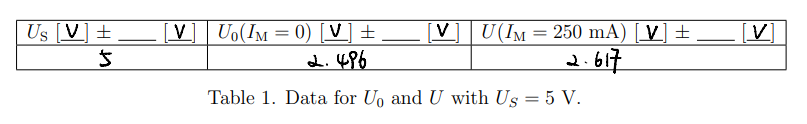
\includegraphics[width=0.7\textwidth]{F1.png}
	%\caption{Data for $U_0$ and $U$ with $U_S$=5V}
	\label{fig1}
\end{figure}
Since the theoretical value of the magnetic field is proportional to the magnitude of $I_M$ when x is a fixed value, 
we can simply acquire the desired value for B by multiplying it by 2.5 times. The calculation is given by:
\begin{equation*}
	B(x=0,I_\text{M}=250\ [\text{mA}]) = \frac{250}{100} \times 1.4366\times10^{-3} = 3.59\times 10^{-3} \pm 0.07 \times 10^{-3}\ \text{T}.
\end{equation*}
Now according to the equation \ref{eq::magnetic field}, we have the following: 
\begin{equation*}
	K_\text{H} = \frac{U-U_0}{B(x=0,I_\text{M}=250\,[\text{mA}])} = \frac{2.617-2.496}{3.59\times 10^{-3}} = 32.86 \,[\text{V}/\text{T}].
\end{equation*}
Thus we get the value desired for the solenoid as $K_H$. It might be used for later calculations.  

\subsection{Relation Between Output Voltage U and Magnetic Field B}
\indent

For the second measurement, we obtain the following data table: 

\begin{figure}[htbp]
	\centering
	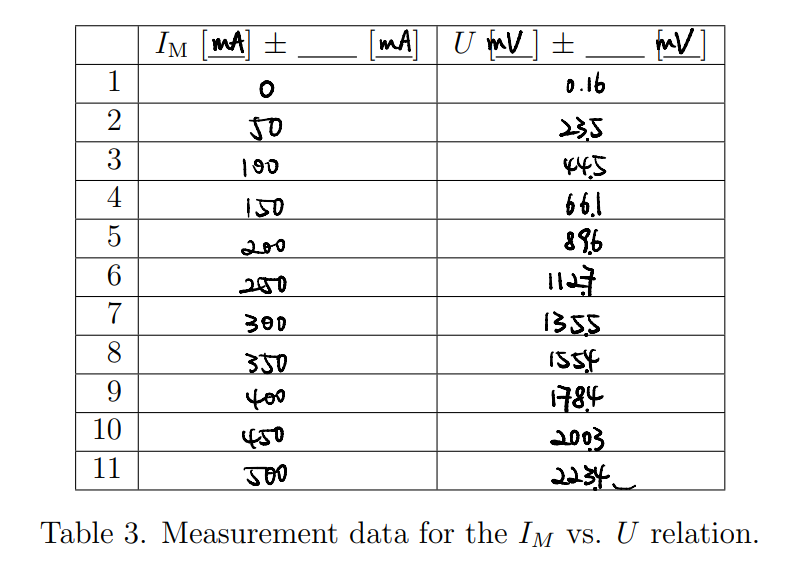
\includegraphics[width=0.9\textwidth]{F2.png}
	%\caption{Data for $U_0$ and $U$ with $U_S$=5V}
	\label{fig2}
\end{figure}
Here again, we notice that the theoretical value of the magnetic field is proportional to the magnitude of $I_M$ when x is a fixed value, and since the measured
$U_out$ is the amplified output of $U_H$ so we suppose that $U = k·U_H $. Thus, we should derive a function given as below:
\begin{equation}
	B(x=0)=k\times \frac{U_H}{K_H}
\end{equation}

We clearly see that B should be proportional to the Hall voltage $U_H$, and this is the relationship we wanted to discover in this part. 
To find the value of $K_H$, we can apply a linear fit to the data of $I_M$ and $U_H$. Notice that we have the following equation:
\begin{equation*}
	B(x) = \mu_0\frac{N}{L}I_\text{M}\left(\frac{L+2x}{2[D^2+(L+2x)^2]^{\frac{1}{2}}}+\frac{L-2x}{2[D^2+(L-2x)^2]^{\frac{1}{2}}}\right) = C(x)I_\text{M}
\end{equation*}
It is obvious that by moving the terms around, we will eventually have $K_H$ as some multiple of slope of $I_M$ v.s $U_H$。 The linear fit is shown below:
\begin{figure}[htbp]
	\centering
	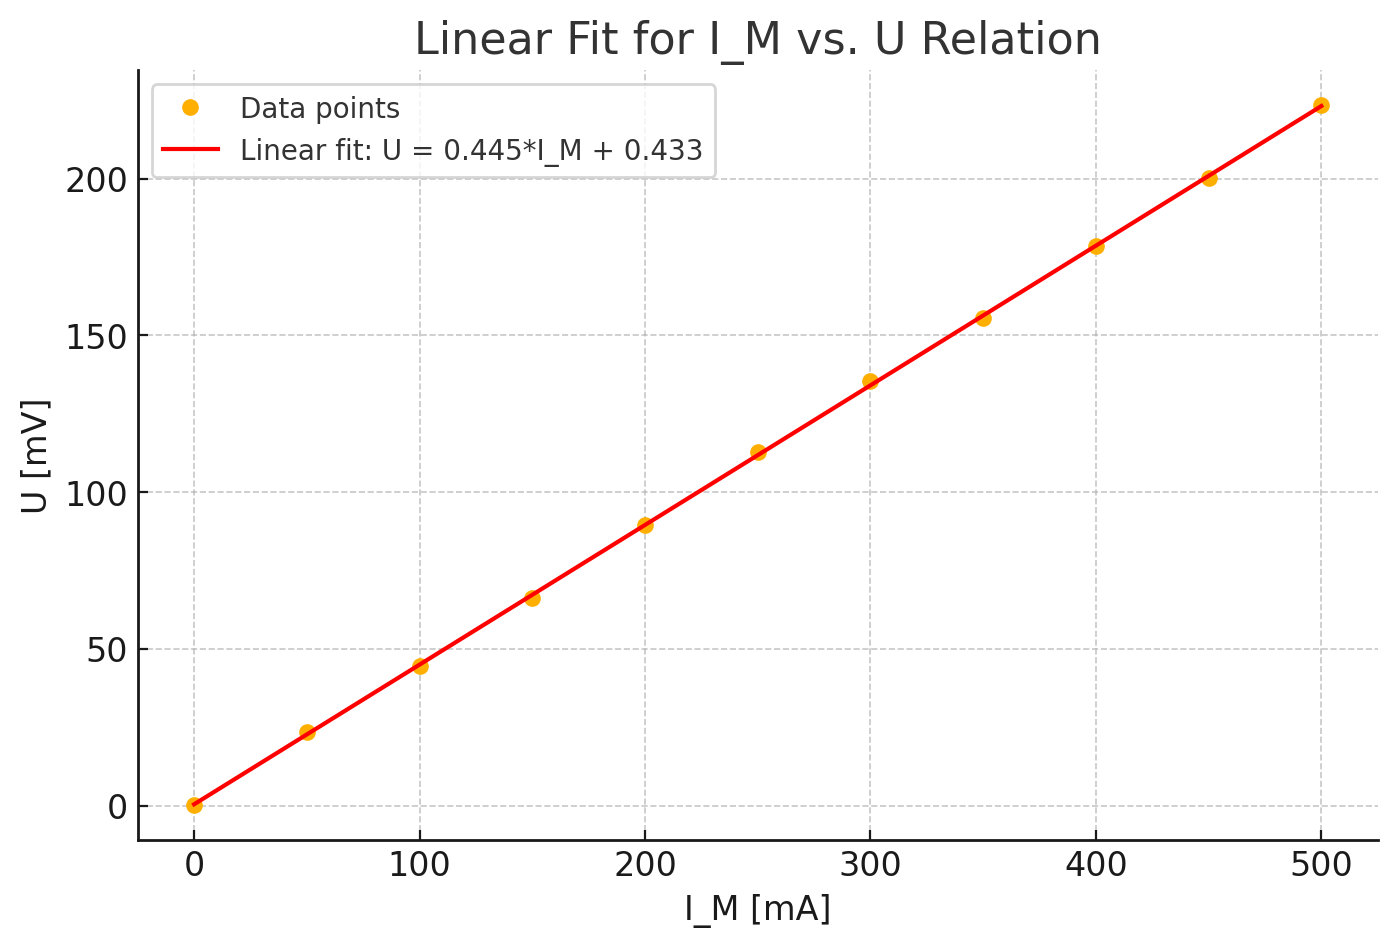
\includegraphics[width=0.9\textwidth]{F4.png}
	%\caption{Data for $U_0$ and $U$ with $U_S$=5V}
	\label{fig2}
\end{figure}
We have mentioned before that the magnitude of $I_M$ is proportional to the magnitude of B at x=0, so we will have the following equation:
\begin{equation*}
	B(x=0)=\frac{I_M}{100}\times1.4366\times10^{-3}
\end{equation*}
After transferring the original slope of $I_M$ and $U_H$, we get the value of $K_H$ to be around $33.01 \,[\text{V}/\text{T}].$

\subsection{Magnetic Field Distribution Inside the Solenoid}
\indent

For the third measurement, we obtain the following data table: 

\begin{figure}[htbp]
	\centering
	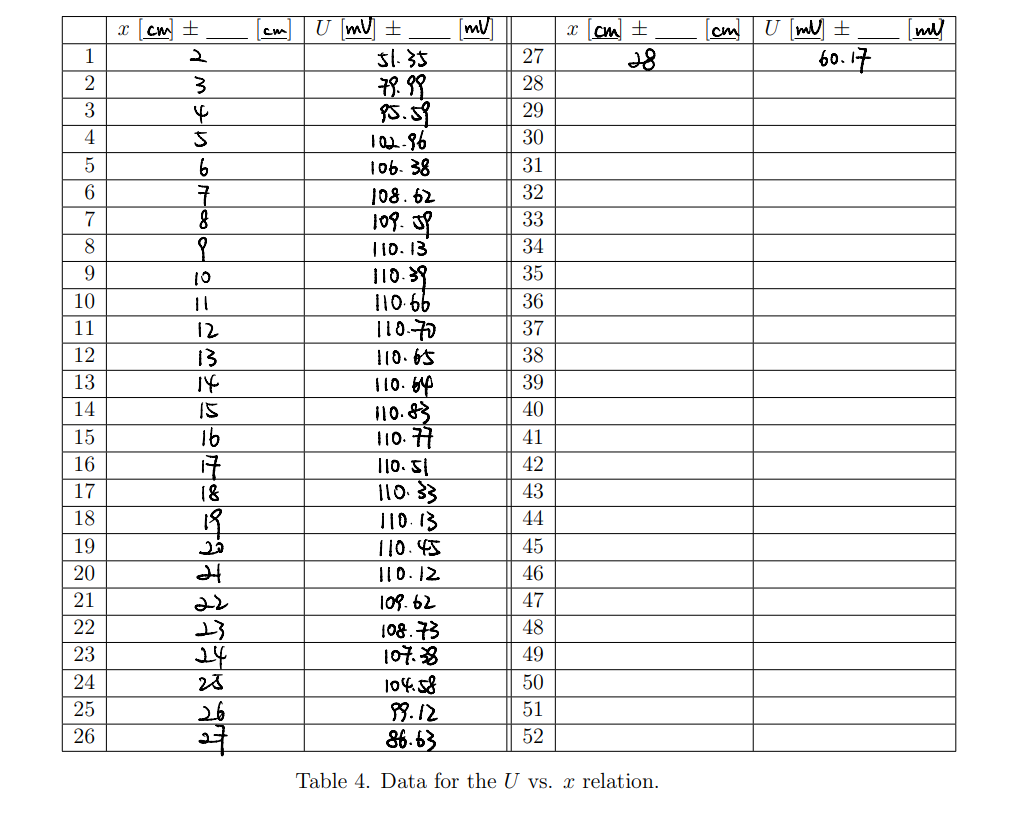
\includegraphics[width=0.9\textwidth]{F3.png}
	%\caption{Data for $U_0$ and $U$ with $U_S$=5V}
	\label{fig4}
\end{figure}

Here we want to look at the distribution of magnetic field inside the tube, so we will use this equation for calculation:
\begin{equation}
	B(x)=\frac{U}{K_H}
\end{equation}
In this equation, the value of $K_H$ will be the value calculated in the section before. We wwill plot both the measured and theoratical values 
of magnetic field distribution in one single figure
\begin{figure}[htbp]
	\centering
	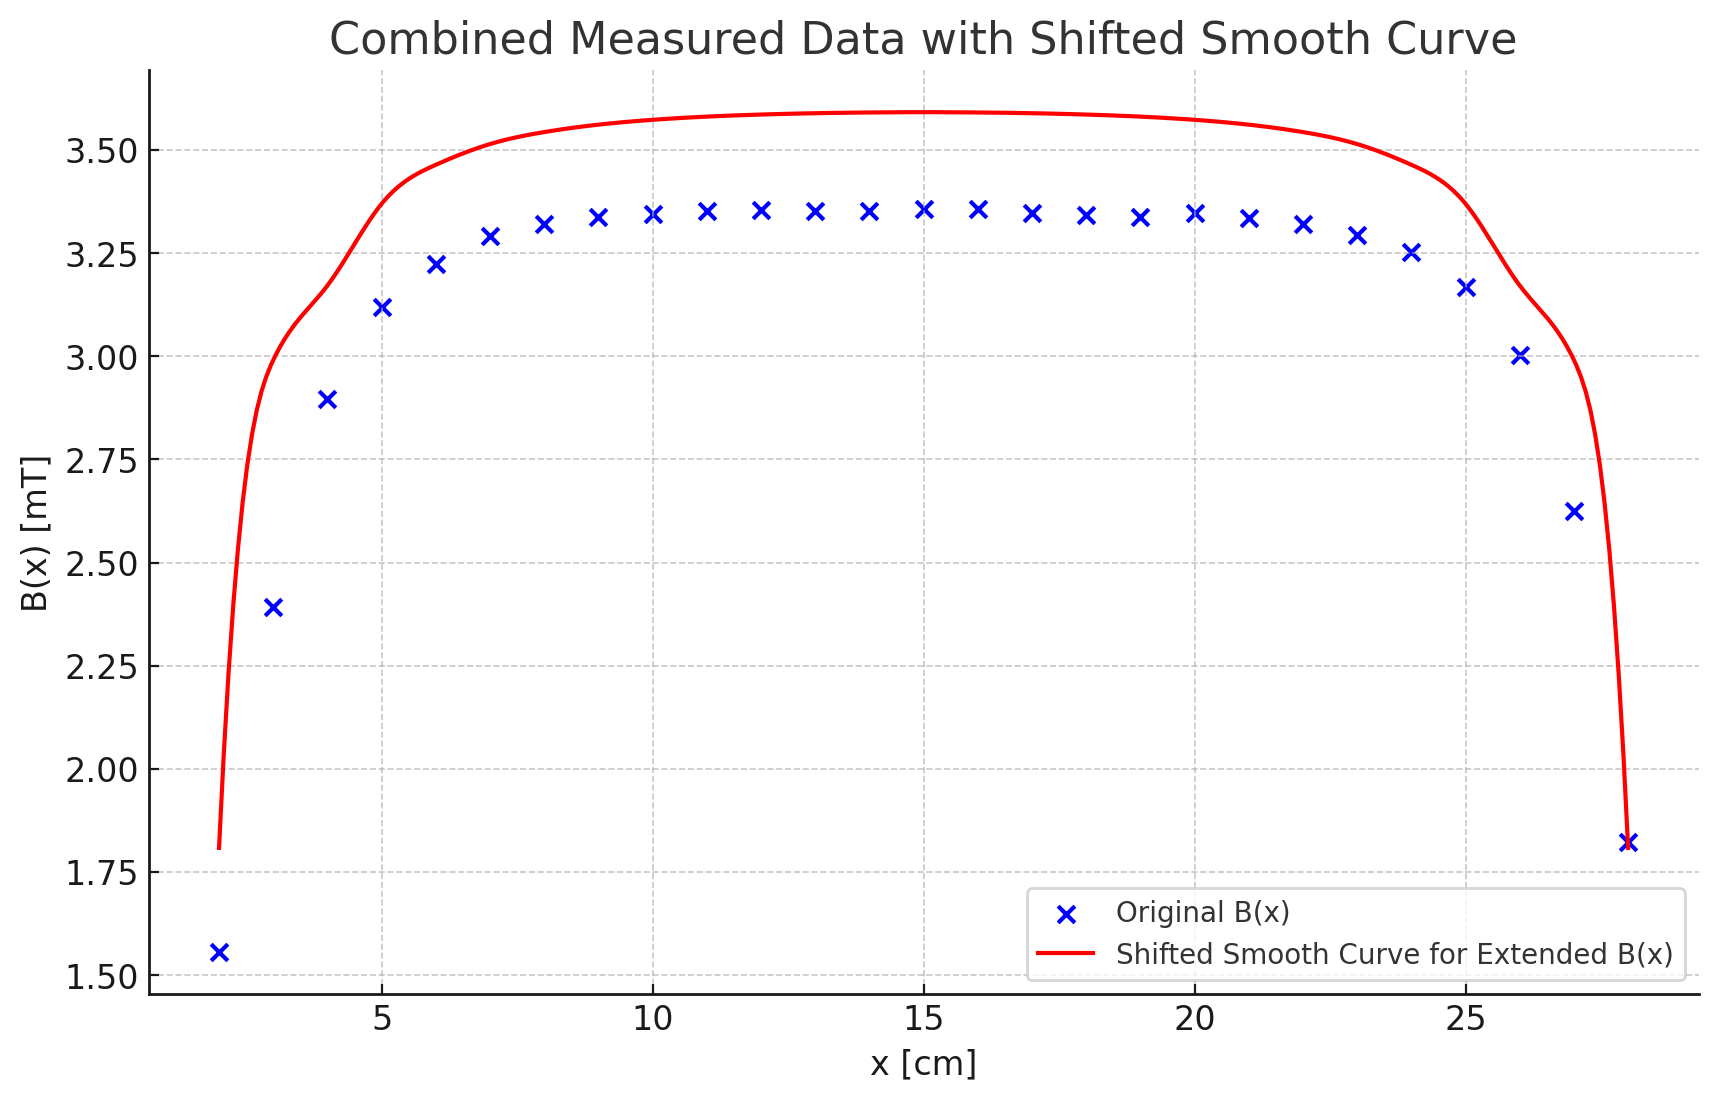
\includegraphics[width=0.9\textwidth]{F5.png}
	%\caption{Data for $U_0$ and $U$ with $U_S$=5V}
	\label{fig5}
\end{figure}
From the figure we see that the measured values are quite close to the theoratically desired value. 

\section{Conclusions and discussion}
\indent

\subsection{H-B Curve and desired values of data}
\indent

In this experiment, we developed a rough idea about how to use integrated Hall probe and measured its sensitivity under different
working voltages. We also measured two values for $K_H$ using both direct calculation and linear fit, and compared them with each other.
Also, we took the data needed to calculate the magnetic field distribution inside a solenoid.

From the results of the experiment, we can see that the sensitivity is decreasing as the working voltage increases. Also, the distribution 
of magnetic field inside a solenoid has the characteristic of having the maximum near the mid point, and gradually decreases along 
the axis with increasing rate. All these help us learn about the Hall probe better.

\subsection{Discussion}
\indent

There are still some errors with magnitude that can not be ignored, and we here briefly discuss some possible reasons. The most significant
reason might be due to the errors generated by the equipments themselves. During the experiment, we noticed that the reading of some values
such as the working voltage kept changing rapidly. This to some extent greatly affected the accurate reading of the working voltage. Other factors 
may also involve problems such as uneven probe etc. However, all the problems are minor issues and can be easily solved by small improvements
to the experiment. 

\section{Works cited}
Department of Physics, Shanghai Jiaotong University, Exercise 2 (The Hall Probe: Characteristics and Applications) - lab manual [rev. 3.9], 2024\\
Python Software Foundation. (2020). Python Language Reference, version 3.9. Available at http://www.python.org\\
\\
All the figures displayed in the article (excluding the appendix) are given using Python 3.9.
\pagebreak
\appendix
\section{Datasheet}

\begin{figure}[htbp]
	\centering
	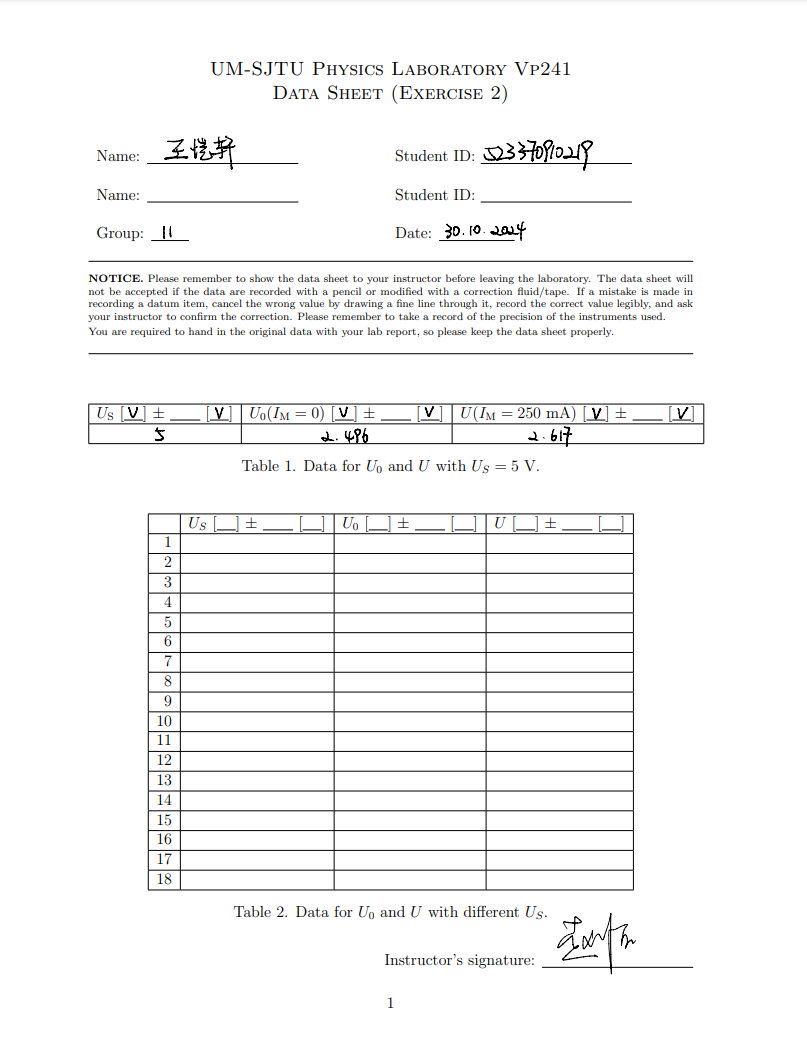
\includegraphics[width=0.9\textwidth]{D1.png}
	%\caption{Data for $U_0$ and $U$ with $U_S$=5V}
	\label{fig5}
\end{figure}

\begin{figure}[htbp]
	\centering
	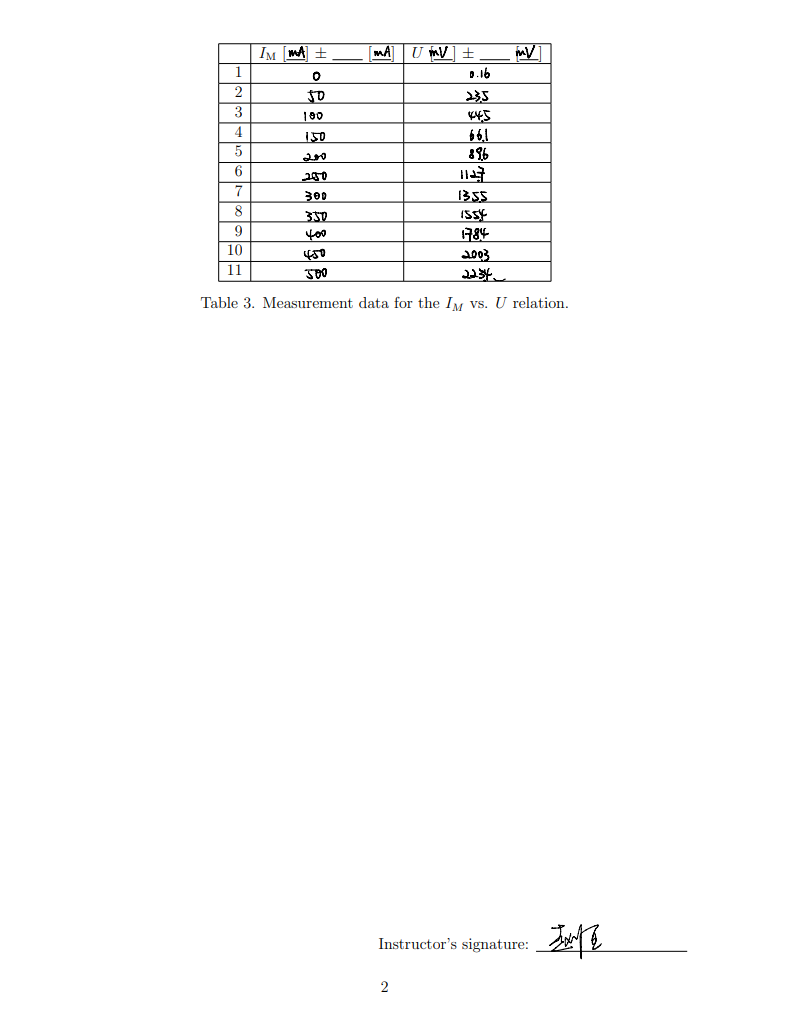
\includegraphics[width=0.9\textwidth]{D2.png}
	%\caption{Data for $U_0$ and $U$ with $U_S$=5V}
	\label{fig5}
\end{figure}

\begin{figure}[htbp]
	\centering
	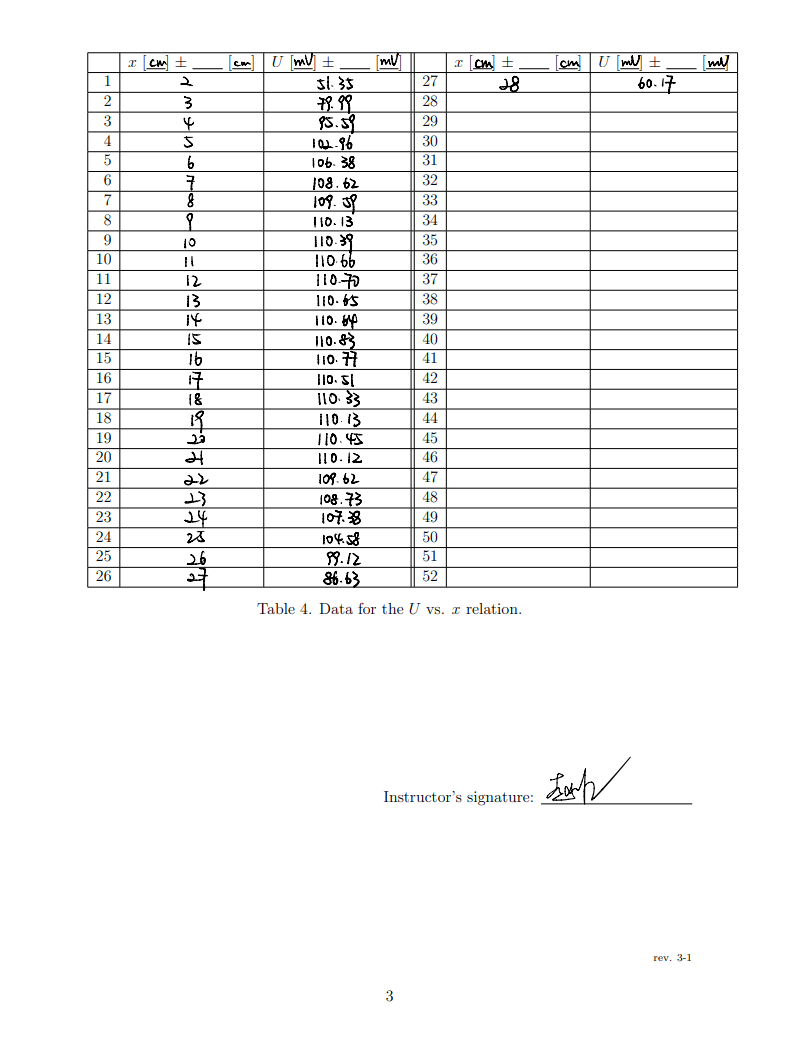
\includegraphics[width=0.9\textwidth]{D3.png}
	%\caption{Data for $U_0$ and $U$ with $U_S$=5V}
	\label{fig5}
\end{figure}

%\textcolor{blue}{Please remember to attach the original data sheet signed by your instructor.}
\end{document}